\documentclass[14pt]{extarticle}
\usepackage[utf8]{inputenc}
\usepackage[T1]{fontenc}
\usepackage[spanish,es-lcroman]{babel}
\usepackage{amsmath}
\usepackage{amsthm}
\usepackage{physics}
\usepackage{tikz}
\usepackage{float}
\usepackage[autostyle,spanish=mexican]{csquotes}
\usepackage[per-mode=symbol]{siunitx}
\usepackage{gensymb}
\usepackage{multicol}
\usepackage{enumitem}
\usepackage[left=2.00cm, right=2.00cm, top=2.00cm, 
     bottom=2.00cm]{geometry}
\usepackage{Estilos/ColoresLatex}

\newcommand{\textocolor}[2]{\textbf{\textcolor{#1}{#2}}}

%\renewcommand{\questionlabel}{\thequestion)}
\decimalpoint
\sisetup{bracket-numbers = false}

\title{\vspace*{-2cm} Ejercicios Opcionales Solución- Física 1\vspace{-5ex}}
\date{\today}

\begin{document}
\maketitle

\section{Ejercicios a cuenta}

\begin{enumerate}
\item Realizar la conversión de \SI{7}{\square\meter} a pie$^{2}$.

\textbf{Solución:}
\begin{align*}
1 \, \text{pie} &= \SI{0.3048}{\meter} \\[0.5em]
\left( 1 \, \text{pie} \right)^{2} &= \left( \SI{0.3048}{\meter} \right)^{2} \\[0.5em]
1 \, \text{pie}^{2} &= \SI{0.0929}{\square\meter} \\[0.5em]
\left(\SI{7}{\square\meter}  \right) \left( \dfrac{1 \, \text{pie}^{2}}{\SI{0.0929}{\square\meter}} \right) &= 75.34 \, \text{pie}^{2} 
\end{align*}
\item Una lancha de motor efectúa los siguientes desplazamientos: \SI{300}{\meter} al oeste, \SI{200}{\meter} al norte, \SI{350}{\meter} al noreste y \SI{150}{\meter} al sur.
\begin{enumerate}[label=\alph*)]
\item ¿Qué distancia total recorre?
\item Determina gráficamente, ¿cuál es su desplazamiento resultante, en qué dirección actúa, y cuál es el valor de su ángulo medido respecto al oeste? Tendrás que hacer uso de tu juego de geometría y de preferencia en un papel cuadriculado.
\end{enumerate}

\textbf{Solución:}
\begin{enumerate}
\item La distancia que recorre la lancha es:
\begin{align*}
d = \SI{300}{\meter} + \SI{200}{\meter} + \SI{350}{\meter} + \SI{150}{\meter} = \SI{1000}{\meter}
\end{align*}
\item El desplazamiento resultante de la lancha es de \SI{300}{\meter} en dirección noroeste, que forma un ángulo de \ang{80.5} medido con respecto al oeste.
\begin{figure}[H]
    \centering
    \begin{tikzpicture}
        \draw (-4, 0) -- (3, 0) node [above, pos=1] {\small{$x \, [\unit{\meter}]$}};
        \draw (0, -0.5) -- (0, 5) node [right, pos=1.1] {\small{$y \, [\unit{\meter}]$}};

        \draw [-stealth, thick, color=blue] (0, 0) -- (-3, 0) -- (-3, 2) -- (-0.52, 4.47) -- (-0.52, 2.97);
        \draw [-stealth, thick, color=red] (0, 0) -- (-0.52, 2.97);
        \draw [red, thick] (-0.5, 0) arc(180:100:0.5);
    \end{tikzpicture}
\end{figure}

\end{enumerate}
\item Con una cuerda, un niño jala un carro con una fuerza de \SI{80}{\newton}, la cual forma un ángulo de $\ang{40}$ con el eje horizontal como se puede observar en la figura:
\begin{figure}[H]
     \centering
     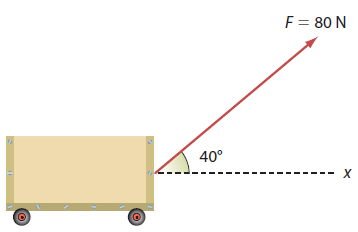
\includegraphics[scale=1]{Imagenes/Ejercicio_Opcional_01.png}
\end{figure}
Calcula:
\begin{enumerate}[label=\alph*)]
\item La magnitud de la fuerza que jala el carro horizontalmente.
\item La magnitud de la fuerza que tiende a levantar al carro.
\end{enumerate}
\textbf{Solución:}
\begin{enumerate}
\item La componente horizontal es:
\begin{align*}
F_{x} = F \, \cos \ang{40} = (\SI{80}{\newton})(0.766) = \SI{61.28}{\newton} \\[0.5em]
\end{align*}
\item La componente vertical es:
\begin{align*}
F_{y} = F \, \sin \ang{40} = (\SI{80}{\newton})(0.6428) = \SI{51.42}{\newton}
\end{align*}
\end{enumerate}

\item Realiza la siguiente operación en notación científica, debiendo de hacer el manejo en todo momento con la notación:
\begin{align*}
\dfrac{\num{6.1d18}}{\num{7.5d7}} + \num{7d9} - \left[ \left( \num{4.51d-5} \right) \left( \num{2.3d-2} \right)\right]
\end{align*}

\textbf{Solución:} Resolvemos primero el paréntesis
\begin{align*}
\left[ \left( \num{4.51d-5} \right) \left( \num{2.3d-2} \right)\right] &= (4.51 \times 2.3) \times 10^{-5+(-2)} = \\[0.5em]
&= \num{10.373d-7} = \num{1.0373d-6}
\end{align*}
Luego resolvemos el cociente:
\begin{align*}
\dfrac{\num{6.1d18}}{\num{7.5d7}} &= \left( \dfrac{6.1}{7.5} \right) \times 10^{18 + (-7)} = \\[0.5em]
&= \num{0.8133d11} = \num{8.133d10}
\end{align*}
Hacemos la suma de los tres términos:
\begin{align*}
\num{8.133d10} + \num{7d9} - \num{1.0373d-6} =
\end{align*}
Igualando en cada término el exponente de la cantidad mayor:
\begin{align*}
&\num{8.133d10} + \num{0.7d10} + \num{0.000000000000000010373d10} = \\[0.5em]
&= \num{8.833d10}
\end{align*}
\item Se desea conocer cuántos litros de agua le caben a una alberca olímpica de \SI{50}{\meter} de largo,
\SI{25}{\meter} de ancho y \SI{2.7}{\meter} de profundidad.

\textbf{Solución:} El problema pide calcular el volumen en litros cúbicos de agua para el volumen de la alberca:
\begin{align*}
V = \SI{50}{\meter} \times \SI{25}{\meter} \times \SI{2.7}{\meter} = \SI{3375}{\cubic\meter}
\end{align*}
Lo que falta es obtener la equivalencia entre metros cúbicos y litros:
\begin{align*}
\SI{1}{\cubic\meter} = \SI{1000}{\liter}
\end{align*}
Así tenemos:
\begin{align*}
\SI{3375}{\cubic\meter} \left( \dfrac{\SI{1000}{\liter}}{\SI{1}{\cubic\meter}} \right) = \SI{3.375d6}{\liter}
\end{align*}
\end{enumerate}

\end{document}